\documentclass[12pt]{article}
\usepackage[margin=3cm]{geometry}
\usepackage{graphicx}
\usepackage{float}
\usepackage{url}
\usepackage{listings}
\usepackage{color}

\definecolor{mygreen}{rgb}{0,0.6,0}
\definecolor{mygray}{rgb}{0.5,0.5,0.5}
\definecolor{mymauve}{rgb}{0.58,0,0.82}
\lstset{ %
	xleftmargin=15em,
	backgroundcolor=\color{white},   % choose the background color; you must add \usepackage{color} or \usepackage{xcolor}
	basicstyle=\small,%\footnotesize,        % the size of the fonts that are used for the code
	breakatwhitespace=false,         % sets if automatic breaks should only happen at whitespace
	breaklines=false,                 % sets automatic line breaking
	captionpos=b,                    % sets the caption-position to bottom
	commentstyle=\color{mygreen},    % comment style
	deletekeywords={...},            % if you want to delete keywords from the given language
	escapeinside={\%*}{*)},          % if you want to add LaTeX within your code
	extendedchars=true,              % lets you use non-ASCII characters; for 8-bits encodings only, does not work with UTF-8
	%	frame=single,                    % adds a frame around the code
	keepspaces=true,                 % keeps spaces in text, useful for keeping indentation of code (possibly needs columns=flexible)
	keywordstyle=\color{blue},       % keyword style
	language=C, % the language of the code
	morekeywords={*,...},            % if you want to add more keywords to the set
	numbers=left,                    % where to put the line-numbers; possible values are (none, left, right)
	numbersep=5pt,                   % how far the line-numbers are from the code
	numberstyle=\small\color{mygray}, % the style that is used for the line-numbers
	rulecolor=\color{black},         % if not set, the frame-color may be changed on line-breaks within not-black text (e.g. comments (green here))
	showspaces=false,                % show spaces everywhere adding particular underscores; it overrides 'showstringspaces'
	showstringspaces=false,          % underline spaces within strings only
	showtabs=false,                  % show tabs within strings adding particular underscores
	stepnumber=1,                    % step between two line-numbers. If it's 1, each line will be numbered
	stringstyle=\color{mymauve},     % string literal style
	tabsize=2                  % sets default tabsize to 2 spac                  % show the filename of files included with \lstinputlisting; also try caption instead of title
}

\begin{document}

\begin{titlepage}
	\begin{center}
		
		
		% Upper part of the page. The '~' is needed because \\
		% only works if a paragraph has started.
		\vfill
		
		\textsc{\LARGE Lab 7: Carry-Ripple Addition II}\\[1.5cm]
		
		\Large Adam Sumner\\[0.5cm]
		
		\Large Illinois Institute of Technology\\[0.5cm]
		
		\Large ECE 429-01\\[0.5cm]	
		
		\noindent
		\vfill
		\large \textbf{Lab Date:} October 26\textsuperscript{th}, 2015\hfill
		\large \textbf{Due Date:} November 2\textsuperscript{nd}, 2015
		% Bottom of the page
	
		
	\end{center}
\end{titlepage}

\section{Introduction}
The purpose of this lab is to continue the design process of the carry-ripple adder from lab 6. Specifically, the layout of the carry-ripple adder will be designed and implemented. It will then be verified using Design Rule Checking (DRC) and Layout v.s. Schematic Verification (LVS).
\section{Theory/Pre-Lab}
\subsection{Theory}
When designing the layout of a large or complex circuit, it is incredibly important to be meticulous so that too many design rules are not violated when the layout is complete. Many errors in the layout design will result in an extremely difficult process of correction. Using the reference design shown in Figure \ref{fig:ref} as a design rule guideline, the stick diagram can easily be built with minimal errors. Figures \ref{fig:pre-1} - \ref{fig:pre-5} show the stick diagrams for the full adder.

\begin{figure}[H]
\centering
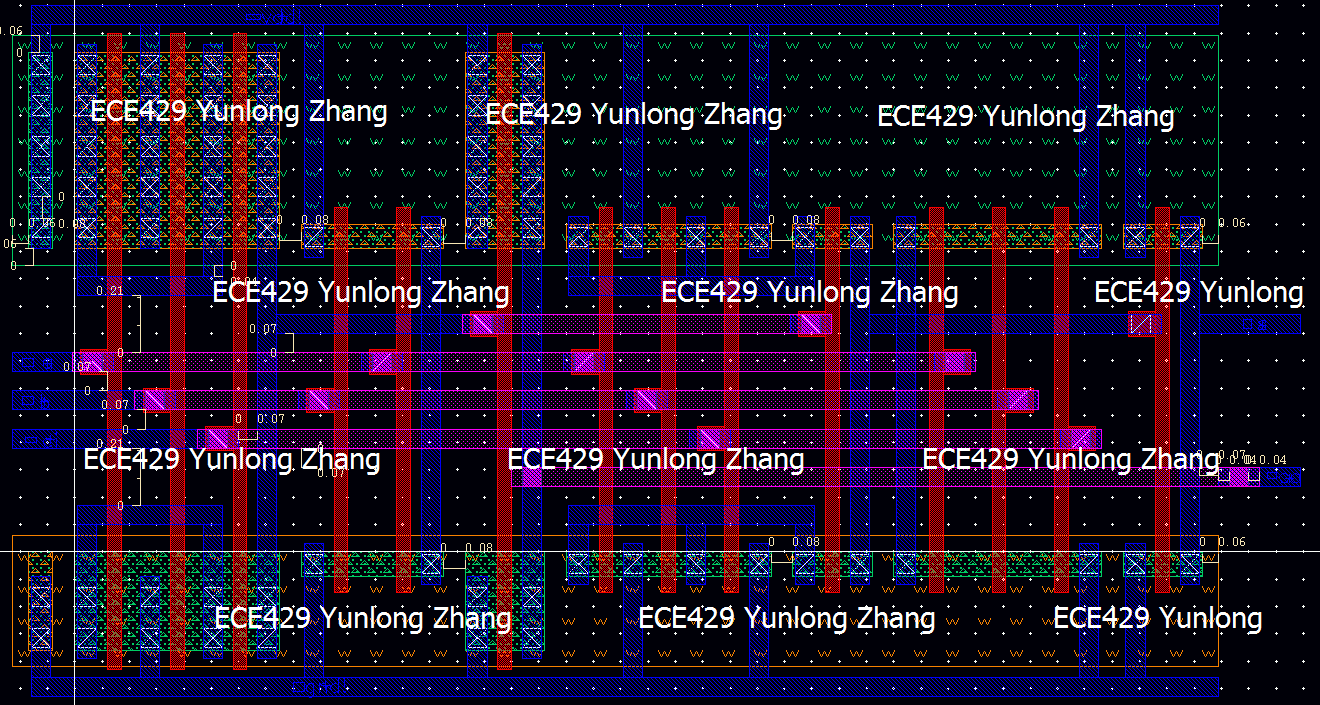
\includegraphics[width=\linewidth]{ref}
\caption{Reference Mirror Adder Layout}
\label{fig:ref}
\end{figure}

\subsection{Pre-Lab}
Due to the size of the layout of this circuit, the sketch of the stick diagram was separated into the individual parts of the schematic. This was done to accurately show the connections involved in this circuit due to the fact that layers of metal cannot be easily drawn using pen and paper. The original schematic is shown in Figure \ref{fig:mirror-schemat}.
\begin{figure}[H]
\centering
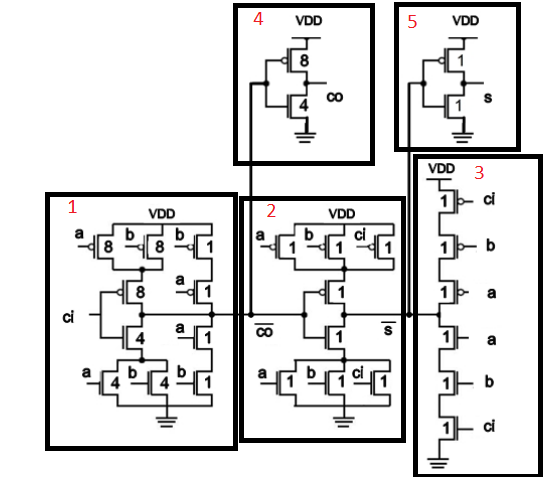
\includegraphics[width=0.7\linewidth]{mirror-schemat}
\caption{Mirror Adder Schematic}
\label{fig:mirror-schemat}
\end{figure}


\begin{figure}[H]
\centering
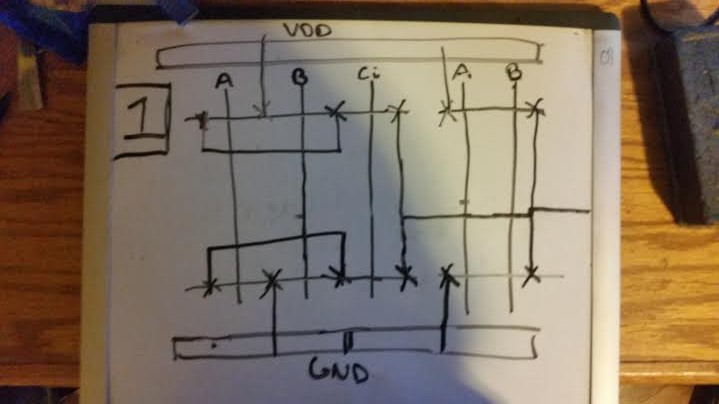
\includegraphics[width=0.7\linewidth]{pre-1}
\caption{Section 1}
\label{fig:pre-1}
\end{figure}

\begin{figure}[H]
\centering
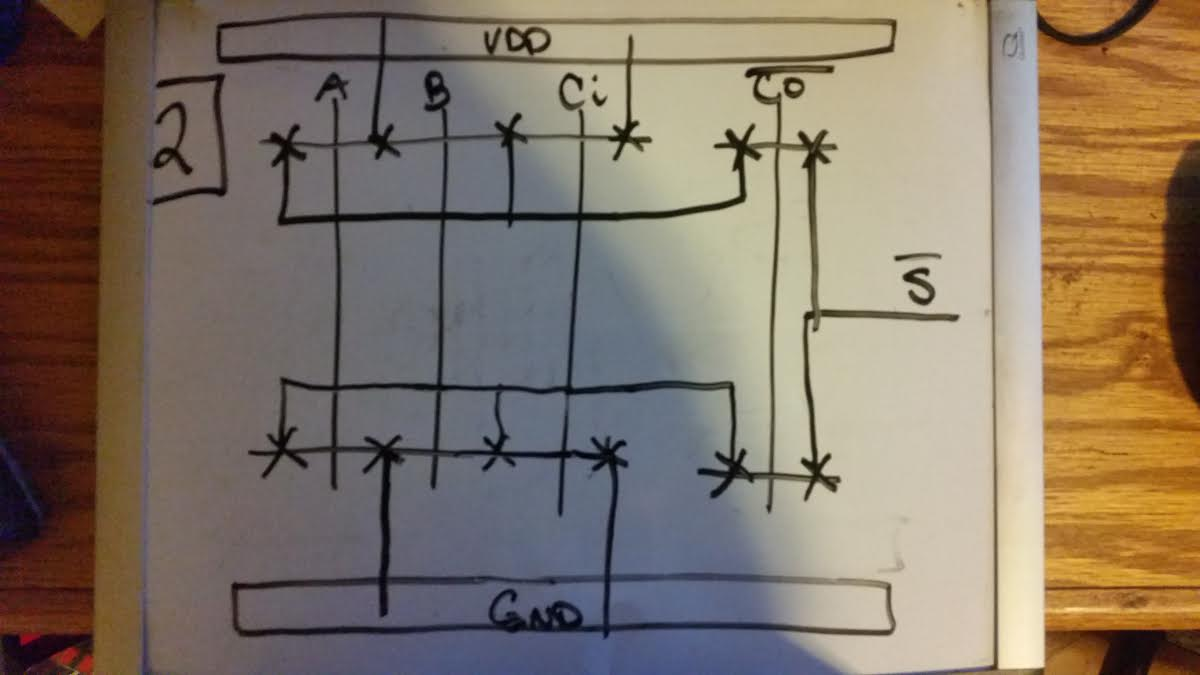
\includegraphics[width=0.7\linewidth]{pre-2}
\caption{Section 2}
\label{fig:pre-2}
\end{figure}

\begin{figure}[H]
\centering
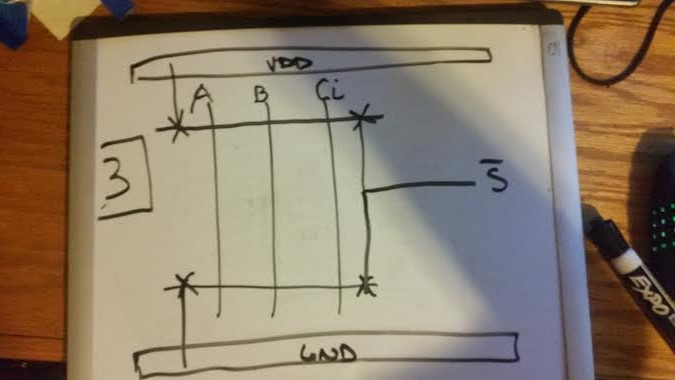
\includegraphics[width=0.7\linewidth]{pre-3}
\caption{Section 3}
\label{fig:pre-3}
\end{figure}


\begin{figure}[H]
\centering
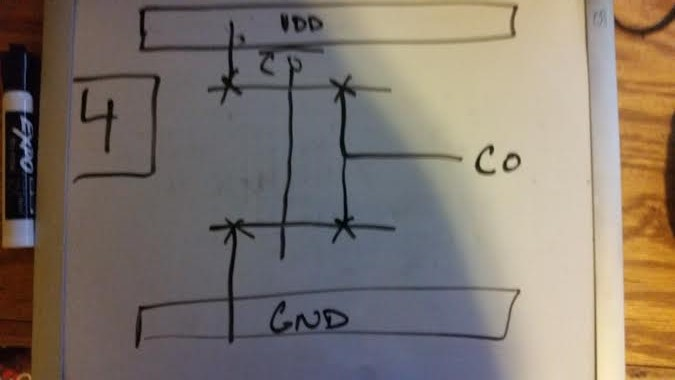
\includegraphics[width=0.7\linewidth]{pre-4}
\caption{Section 4}
\label{fig:pre-4}
\end{figure}

\begin{figure}[H]
\centering
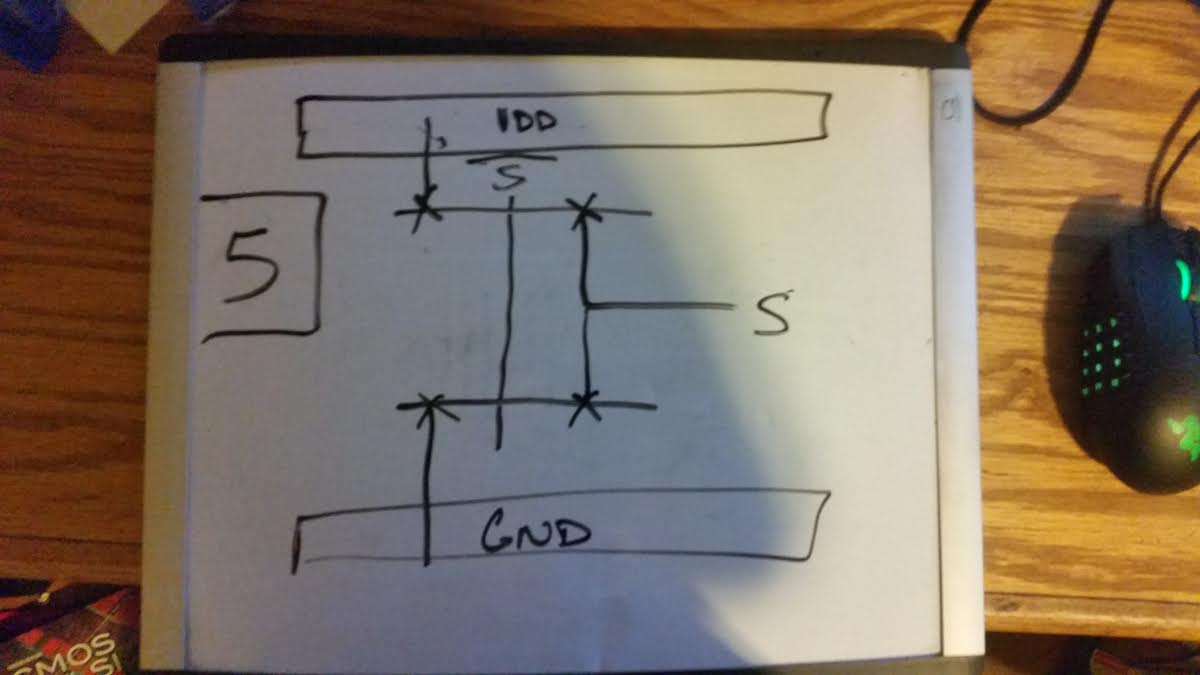
\includegraphics[width=0.7\linewidth]{pre-5}
\caption{Section 5}
\label{fig:pre-5}
\end{figure}


\section{Implementation}
\subsection{Schematics}
\begin{figure}[H]
\centering
\caption{Implemented Layout of Mirror Adder}
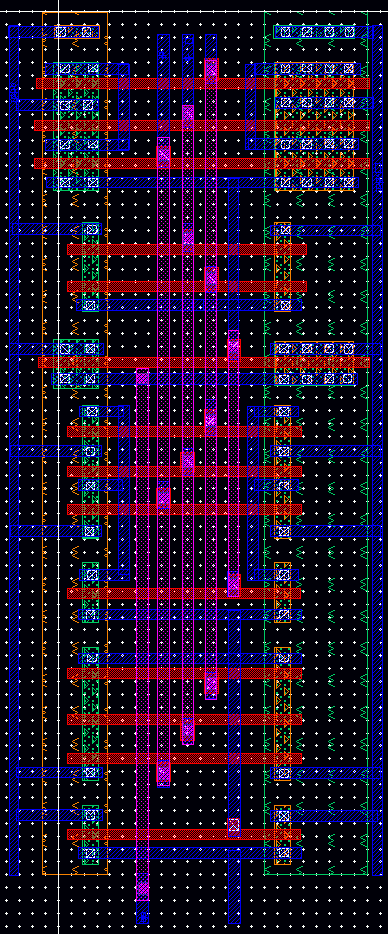
\includegraphics[width=\textwidth,height=\textheight,keepaspectratio]{layout}

\label{fig:layout}
\end{figure}

\subsection{Procedure}
First the layout of the full adder was constructed. After several hours of hard meticulous work and constant DRC to make sure the design followed the guidelines, LVS was performed and any errors were corrected until the smiley face was generated. 
\subsection{Results}
\begin{figure}[H]
\centering
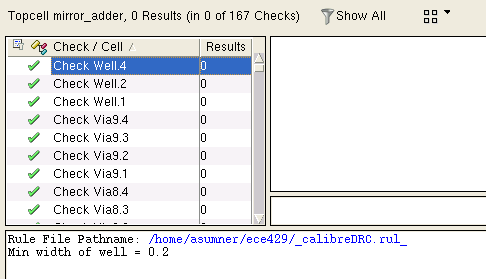
\includegraphics[width=1\linewidth]{drc}
\caption{DRC Verification}
\label{fig:drc}
\end{figure}

\begin{figure}[H]
\centering
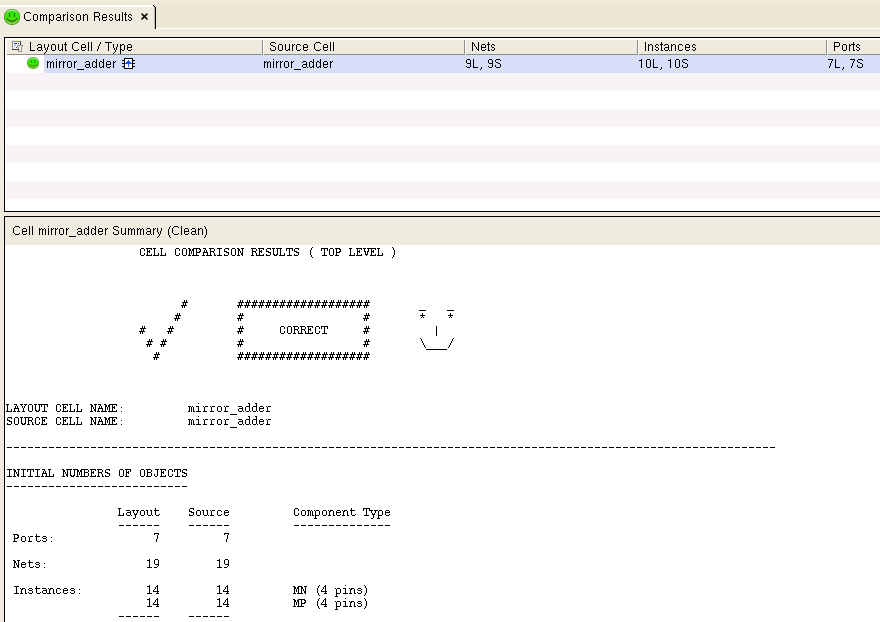
\includegraphics[width=1\linewidth]{lvs}
\caption{LVS Verification}
\label{fig:lvs}
\end{figure}



\subsection{Discussion}
While this lab did not seem to have a long procedure, the physical construction of the layout to minimize the size of the design took several hours (5+). Upon construction and verification of the design, it was noted that the focus needed to be a competent VLSI design engineer is quite intense. Luckily, the hard work paid off as Figures \ref{fig:drc} and \ref{fig:lvs} demonstrate the successful work completed in this lab. In order to succeed in layout design, constant DRC must be utilized. It's incredibly easy to misplace an object by 1 nm, which in turn can lead to a lot of DRC errors later on if not caught early. The key to layout design is patience, great planning skills, and an appetite for paying attention to close detail. 
%\subsection{Bonus Work}
\section{Conclusions}
Overall this lab was a success. The layout of the mirror adder was completed and its functionality was successfully verified. It may now be used in future designs, such as constructing a 4-bit adder. 

\end{document}
